%!TEX root = ../../thesis.tex

%=============================================================================


\section{Library}
\label{main:lib}
In this part of our work we will describe the library of our proposed pipeline, along with its tasks.
As discussed earlier, the library of our proposed pipeline solves a number of problems, which are either directly needed for synchronization of results or make it considerably easier.
First we will lay down the reasoning for some major design decision.
After this we will go into more detail with more technical explanations.


% audio transmission
One of the central tasks of the library involves transmitting audio from component to component.
This includes some aspects not immediately obvious.
One of those is the audio format each component requires.
An audio format determines the structure of the audio data on a lower level.
Typically, the structure of any audio data can be described by four factors:
\begin{enumerate}
	\item Its \textit{Samplerate}, which determines the resolution of an audio signal is in time domain.
	\item Its \textit{Bitrate}, which determines the resolution of the singular data points within a audio signal.
	\item Its \textit{Endianness}, which determines the order of bytes of the singular data points within a audio signal. Litte-endian encoding puts the least significant bytes first, while big-endian encoding puts the most significant bytes first. 
	\item Its \textit{Channel Count}, which determines the number of distinct audio signals within the signal. When recording audio, the \textit{Channel Count} is generally equivalent to the number of microphones used to record the audio signal.
\end{enumerate}
Working on audio data which is present in a different format then expected will in most cases lead to unusable results, maybe even to critical segmentation faults. 

Under normal circumstances, a component will request audio in the format it requires directly, e.g. via \gls{alsa}.
However, as our library now handles all audio transmission, this is no longer feasible.
With respect to one of our secondary goals, to provide a modular framework, we can also not assume every components algorithm to work with a specific audio format.
This leaves us to either require each component to use a single, pre-determined audio format or resampling and converting audio signals for each component.
By handling resampling and converting of audio signals within the library, components of the resulting framework can theoretically employ any kind of algorithm they desire, without having to handle resampling and converting audio themselves.
Furthermore, by abstracting resampling and converting from the components themselves, the library can be equipped to change audio formats adaptively when new components are introduced or old components vanish from a specific configuration, in a standardized way.

Consequently, the library needs to be able to resample and convert audio between arbitrary audio formats.
We chose the \gls{soxr} library (todo cite), to resample the audio and use a custom implementation to change its \textit{Bitrate} and \textit{Channel Count}.
We prepared the library to handle different \textit{Endianness}, but ultimately did not implement such a feature, as different byte order is mostly a historic phenomenon and most modern operating systems, such as Windows, MacOs and most Unix systems, use little-endian encodin.

From the perspective of the library, we can then divide between an externally used format, which is the format in which the component provides or requests audio data to the library; and an internally used format, which is the format in which the audio is transmitted.
Both of these can be identical, but must not be.
As discussed previously in chapter todo, resampling and converting of audio signals should be minimized, so careful consideration is required when choosing the format with which to transmit audio between components.

It is however equally important where these formats are chosen, as it could be done in two ways:
Either in a distributed manner, where all existing components must communicate with each other and come to a single conclusion.
Alternatively they could be determined in a centralized manner, where a single master program will collect information about each component and then based on this information will make a decision.
This was our chosen course of action, which was motivated as follows:
The main advantage of a distributed approach is that it does not rely on an additional program, as does the centralized approach.
It does so however at a cost. 
Due to the nature of the distributed approach each component taking part must have the same information as each other, that is to say each component must have information about at least each other component.
See for example figure \ref{pic:main:lib:central_vs_dist}.
In this scenario of average complexity 
While the communication between \texttt{c\_1} and \texttt{c\_2} is straight forward within the distributed approach, the communication between \texttt{c\_2}, \texttt{c\_3}, \texttt{c\_4} and \texttt{c\_5} becomes quite convoluted.
Additionally, the way in which each format is determined must be deterministic, as each component must come to the same conclusion.
All this results in a not insignificant overhead in both computational load and inter-component communication.

However, as we already always employ an additional program to synchronize our results, namely the Orchestrator, the benefit of the distributed approach becomes negligible.
We thus chose to implement the centralized approach with the Orchestrator as our master component, which determines each components internally used audio format.
We will go into detail how the Orchestrator chooses these formats in the following section \ref{main:orc}.

\begin{figure}[]
	\centering
	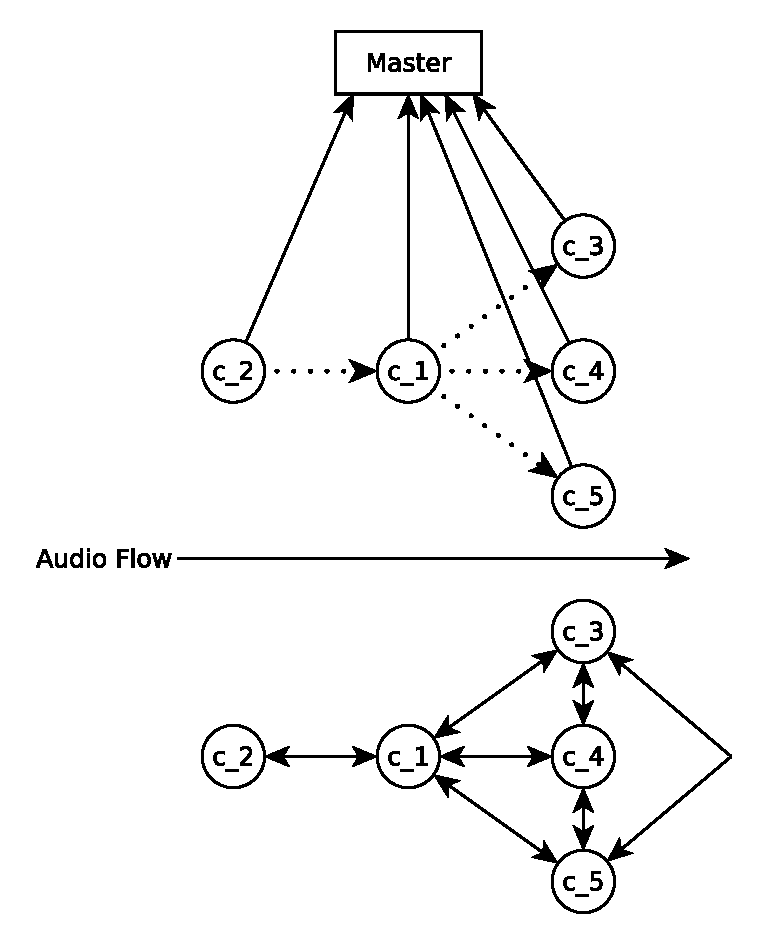
\includegraphics[width=0.66\textwidth]{diagrams/lib_central_vs_dist.pdf}
	\caption{Centralized (above) versus distributed (below) approach of determining audio formats between the components \texttt{c\_1} to \texttt{c\_5}.
		Information sending about each nodes preferred audio topic format are indicated by arrows.
		The direction of audio transmission is indicated by pointed lines above, and from left to right generally speaking.}
	\label{pic:main:lib:central_vs_dist}
\end{figure}

% python bindings
Our library was developed in C++, do to it having access to a number of very widely used and tested libraries for audio processing, such as \gls{sox} as well as its speed.
However, a number of interesting software was developed for Python, see for example libraries on which we based most of our components, discussed below in chapter \ref{main:components:start}.
This is what drove us to develop Python bindings for the library, using Boost Python (todo cite).
It proved fruitful, as most our then developed components actually make use of these bindings rather then the original C++ library.
Developing the library in Python in the first place was considered, but ultimately not chosen because of C++'s superior support with regards to sound libraries, such as \gls{sox} and \gls{soxr}.


%--------------------------------------------------------------------

We will now illustrate the tasks handled by the library by means of typical actions taken by an example component in its life-cycle.
Our example will be that of a typical \gls{vad} component.
As we use \gls{ros} as an underlying middleware, components within the proposed framework must also use \gls{ros} for a number of tasks.
Thus it is necessary for our component to first initialize \gls{ros}.
Following this, the proposed library will need to be initialized, which is done by first creating a handle.
This handle keeps track of all relevant information the proposed library needs.

Our example component may then declare its intention to output or request audio.
In our example, the \gls{vad} component will first declare its intend to output audio and then to require audio.
However, the library does not put a limit as to how many in- \& outputs a component can request, so an identifier is needed.
The same identifier will later internally used to generate the \gls{ros} topics with which the actual audio will be transmitted.
So it also serves to map the audio between components.%todo formulierung
If our \gls{vad} component would use the input topic \texttt{''vad\_input''}, then a microphone component would be needed to output on the same topic, so that the audio could be correctly transmitted.
Also needed to request an audio in- or output is the format in which the audio should arrive or will be given to the library respectively.

When declaring the output of audio, there are no further requirements.
When requesting audio however, the component must present the library with a callback function.
This function will later be invoked when audio was send to the component.

%##########################################

Later, when the component is finished initializing the library and is working, % fomulierung
the component will want to actually receive and output audio.
To output audio, it will need to provide the raw audio signal in the format that it chose previously and its timestamps along with the topic on which this audio shall be transmitted.
The library will then convert this raw audio signal and its corresponding timestamps to a \textit{Augmented Audio Message}, as seen in figure \ref{pic:main:lib:augmented_audio}.
The information contained in these messages can be divided into three categories:
\begin{enumerate}
	\item Transmission information
	\item Synchronization information
	\item Meta information
\end{enumerate}
The transmission information consists of the audio signal to be transmitted as well as an message ID.
This is generated by the library on the transmitting side and is consecutive.
\gls{ros} as a middleware does not ensure messages to arrive at a node in the same order they were sent.
Thus, by adding an ID to each message, the receiving side of the library can later rearrange the order of arrival, should messages arrive out-of-order.
Depending on the size of audio chunk this part of the message should normally be the largest.

The synchronization information is the part of the message which carries the timestamps corresponding to the audio signal.
It therefore enables components to enhance their results with accurate timestamps which in turn are later synchronized by the Orchestrator.

The last part of the 

Conversely, when receiving audio, the library will call the callback function it was given when registering 

In our example \gls{vad} component this may look as follows:


- We will go into detail on how other results are relayed to the Orchestrator below.

\begin{figure}[]
	\centering
	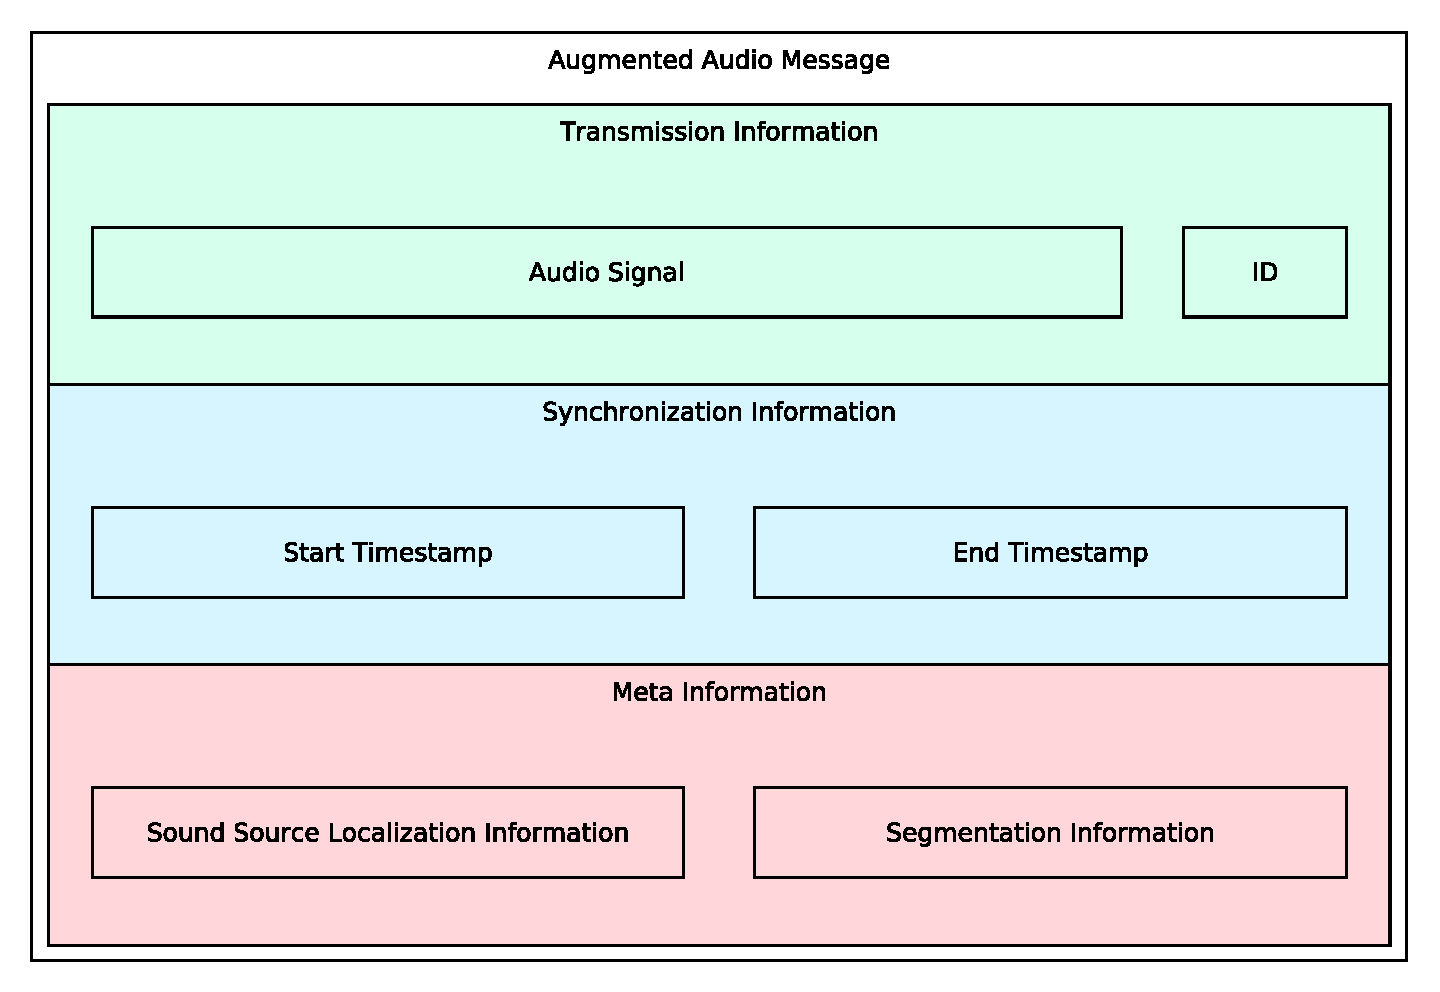
\includegraphics[width=\textwidth]{bilder/rosmsg/augmented_audio.pdf}
	\caption{Composition of Augmented Audio Messages.
		The message can be divided into three parts:
		Transmission information in green, synchronization information in blue, and Meta information in red.}
	\label{pic:main:lib:augmented_audio}
\end{figure}


% ----------------

- actually starting the component

After all these declarations are done, the component will then signal it to the library.
Up until this point, no actual communication between the component and the Orchestrator has happened.
Now however, the library will prepare all information necessary for the Orchestrator to register the component.
Needed is the name of the component, so the Orchestrator can differentiate components from one another, as well the designation of the node, which corresponds to the task the component will perform.
We will go more into detail regarding this designation in the Orchestrator's chapter \ref{main:orc}, as it serves to easy synchronization of results.

Additionally needed are information about the in- \& output topics of audio that were previously declared.
The information about meta-information are not needed for the registration process, as they are handled internally by the library itself.
Registering the component is then done via a dedicated \gls{ros}-service, which has the library send these information
Using a \gls{ros}-service in this instance instead of a simple \gls{ros}-message has the advantage, that we can ensure that the Orchestrator is started and ready, which may not necessarily be the case when starting the Orchestrator and components of the framework in rapid succession.

\begin{figure}[]
	\centering
	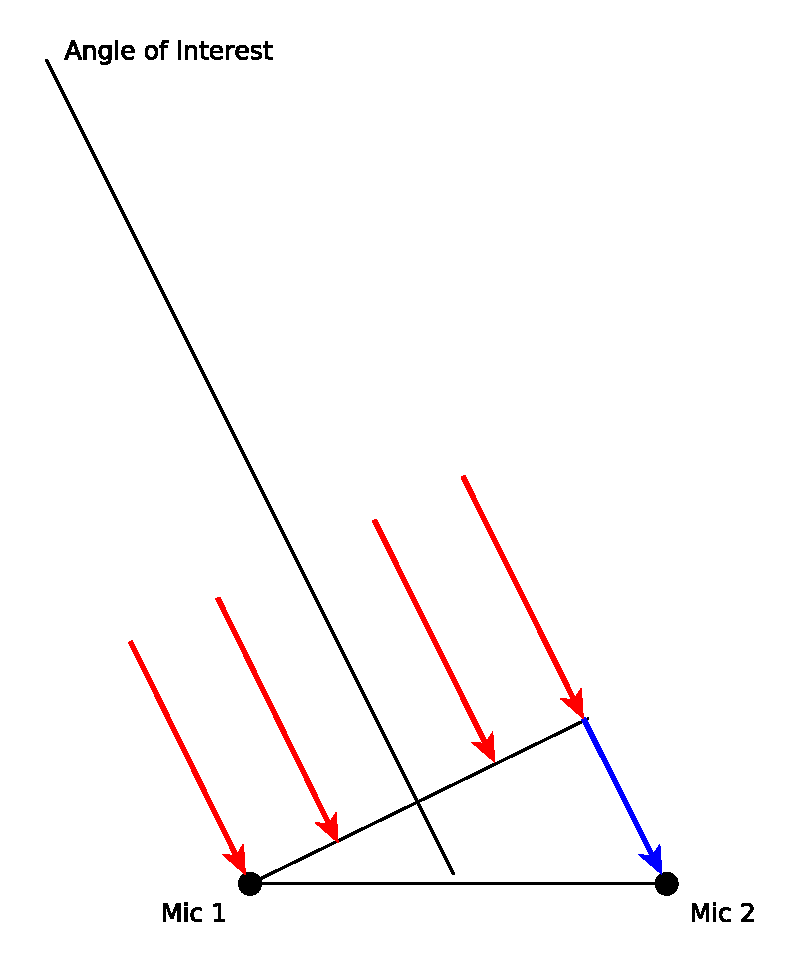
\includegraphics[width=0.66\textwidth]{diagrams/basics_beamforming_2.pdf}
	\caption{}
	\label{pic:main:lib:start_esiaf}
\end{figure}

After this registration has finished, the components work may actually begin.

% ----------------

Components within the framework may or may not generate results based on audio they received.

Thus the library provides standardized \gls{ros}-messages for 
These must then be published manually to similarly standardized \gls{ros}-topics.
This way the Orchestrator can later 

% ----------------

- exiting the component

When the component has finished its work it may provide the library 
, or simply exit.
As we cannot expect the component to 
in all cases, the Orchestrator must be able to handle suddenly disappearing components.
Thus we do not provide a dedicated way to end a component from the perspective of the framework, and instead will focus on the Orchestrator's approach in chapter \ref{main:orc}.


%-------------------------------

- provides standards for
	- audio transmission
		- audio format
		- audio chunk structure
	- node designation
	- announing a node
	- results
	- synchronized results

- handles audio transmission

- handles different audio formats used by the components and seamlessly resamples and converts them.
	- internal formal vs external format

- tasks fulfilled by Orchestrator include
	- determining the best internally used audio format
	- 
	
	
	
% audio grabber as central audio collector
The library was developed to include a number of pre-build components.
In chapter \ref{main:components:start} we will take a closer look into these, among other components.
One of these components however needs to be mentioned here, the \texttt{Audio Grabber}.
It was developed mainly so that no component of the proposed pipeline needs to 
